\chapter{PPP}

\section{Introduction}

HDLC is the default serial encapsulation method when connecting two Cisco routers and it can only work with other Cisco devices. However, when there is a need to connect to a non-Cisco router, PPP encapsulation should be used.\\

There are many advantages to using PPP, including the fact that it is not proprietary. PPP includes many features not available in HDLC: The link quality management feature (LQM) monitors the quality of the link, PPP supports PAP and CHAP authentication.\\

\begin{figure}[hbtp]
\caption{PPP layered architecture}\label{PPPlayers}
\centering
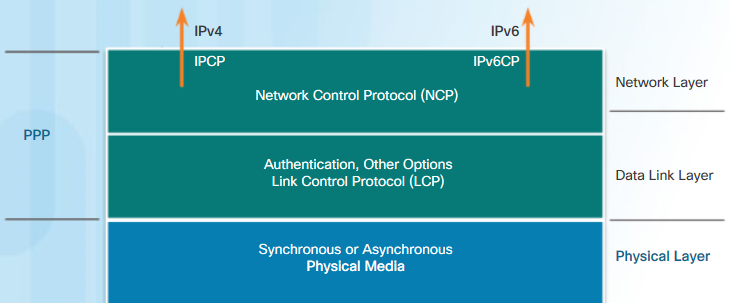
\includegraphics[ width=0.8\textwidth ]{pictures/PPPlayers.PNG}
\end{figure}

PPP contains three main components: HDLC-like framing, LCP, and NCPs. \\

Figure \ref{PPPlayers} maps the layered architecture of PPP against the OSI model. PPP and OSI share the same physical layer, but PPP distributes the functions of LCP and NCP differently. Most of the work done by PPP happens at the data link and network layers, by LCP and NCPs.

\section{Operation}

\subsection{Frame Structure}

A PPP frame consists of six fields. The following descriptions summarize the PPP frame fields illustrated in the figure \ref{PPPframe}: 

\begin{figure}[hbtp]
\caption{PPP Frame fields}\label{PPPframe}
\centering
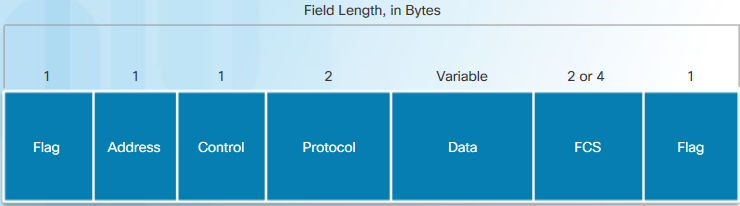
\includegraphics[ width=0.8\textwidth ]{pictures/PPPframe.PNG}
\end{figure}


\begin{itemize}
\item \textbf{Flag:}  A single byte that indicates the beginning or end of a frame. The Flag field consists of the binary sequence 01111110 (63 in decimal). 


\item \textbf{Address:}   A single byte that contains the broadcast address because PPP does not assign individual station addresses. 


\item \textbf{Control:}   A single byte that contains the binary sequence 00000011, which calls for transmission of user data in an unsequenced frame. 

\item \textbf{Protocol:}   Two bytes that identify the protocol encapsulated in the information field of the frame. The 2-byte Protocol field identifies the protocol of the PPP payload.  

\item \textbf{Frame Check Sequence (FCS):} This is 2 bytes. If the receiver’s calculation of the FCS does not match the FCS in the PPP frame, the PPP frame is silently discarded.
\end{itemize}

\subsection{Establishing a PPP Session}

There are three phases of establishing a PPP session, as shown in the figure:

\begin{itemize}
\item \textbf{Phase 1: Link establishment and configuration negotiation} -- The LCP opens the connection and negotiates configuration options. This phase is complete when the receiving router sends a configuration-acknowledgment frame back to the router initiating the connection. 


\item \textbf{Phase 2: Link quality determination (optional)} -- The LCP tests the link to determine whether the link quality is sufficient to bring up network layer protocols. The LCP can delay transmission of network layer protocol information until this phase is complete. 


\item \textbf{Phase 3: Network layer protocol configuration negotiation} -- After the LCP has finished the link quality determination phase, the appropriate NCP can separately configure the network layer protocols. If the LCP closes the link, it informs NCPs so that they can take appropriate action.
\end{itemize}

\subsection{LCP}

Link Control Protocol (LCP) operation uses three classes of LCP frames to accomplish the work of each of the LCP phases: Link-establishment $\rightarrow$ Link-maintenance $\rightarrow$ Link-termination (Figure \ref{PPPEstablishment}).

\begin{figure}[hbtp]
\caption{Establish PPP session: Link-establishment, Link-maintenance, Link-termination}\label{PPPEstablishment}
\centering
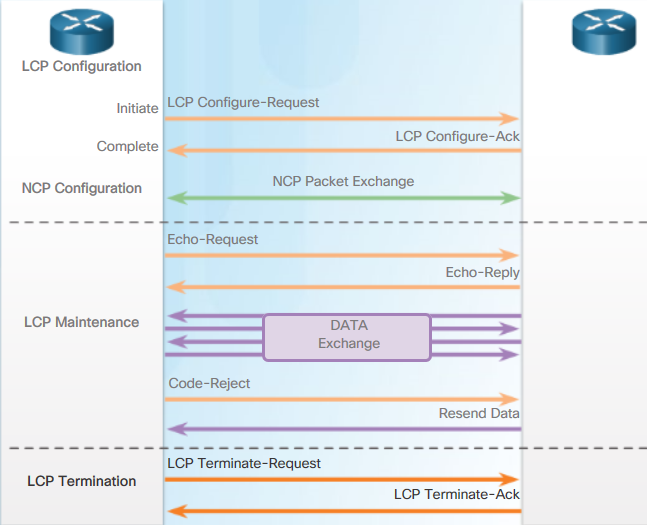
\includegraphics[ width=0.6\textwidth ]{pictures/PPPEstablishment.PNG}
\end{figure}


\subsubsection{Link Establishment}

The link establishment process starts with the initiating device sending a Configure-Request frame to the responder. The initiator includes the options for how it wants the link created, including protocol or authentication parameters. The responder processes the request: 

\begin{itemize}
\item If the options are not acceptable or not recognized, the responder sends a Configure-Nak or Configure-Reject message. If this occurs and the negotiation fails, the initiator must restart the process with new options. 


\item If the options are acceptable, the responder responds with a Configure-Ack message and the process moves on to the authentication stage. The operation of the link is handed over to the NCP.
\end{itemize}

\subsubsection{Link Maintenance}

When NCP has completed all necessary configurations, LCP transitions into link maintenance. During link maintenance, LCP can use messages to provide feedback and test the link using:

\begin{itemize}
\item Echo-Request, Echo-Reply, and Discard-Request: These frames can be used for testing the link.


\item Code-Reject and Protocol-Reject: These frame types provide feedback when one device receives an invalid frame. The sending device will resend the packet.
\end{itemize} 

\subsubsection{Link termination}

After the transfer of data at the network layer completes, the LCP terminates the link, as shown in Figure \ref{PPPEstablishment}. NCP only terminates the network layer and NCP link. The link remains open until the LCP terminates it. If the LCP terminates the link before NCP, the NCP session is also terminated. \\

The LCP closes the link by exchanging Terminate packets. The device initiating the shutdown sends a Terminate-Request message. The other device replies with a Terminate-Ack. 

\subsection{NCP}

After the LCP has configured and authenticated the basic link, the appropriate NCP is invoked to complete the specific configuration of the network layer protocol being used.\\

IPCP is an example of NCP. IPCP is responsible for configuring, enabling, and disabling the IPv4 modules on both ends of the link. IPCP negotiates two options:

\begin{itemize}
\item \textbf{Compression:} Allows devices to negotiate an algorithm to compress TCP and IP headers and save bandwidth.

\item \textbf{IPv4-Address:} Allows the initiating device to specify an IPv4 address to use for routing IP over the PPP link, or to request an IPv4 address for the responder.
\end{itemize}

\subsection{Authentication}

\paragraph{PAP}is a very basic two-way process. There is no encryption. The username and password are sent in plaintext. If it is accepted, the connection is allowed. CHAP is more secure than PAP. PAP may be used in the following environments: CHAP is not supported, or simulate a login at the remote host. \\

\paragraph{PAP Process}After PPP completes the link establishment phase, the remote node repeatedly sends a username-password pair across the link. At the receiving node, the username-password is checked. This device either allows or denies the connection. An accept or reject message is returned to the requester.

\paragraph{CHAP}Unlike PAP, which only authenticates once, CHAP conducts periodic challenges to make sure that the remote node still has a valid password value. The password value is variable and changes unpredictably while the link exists. Thus, CHAP provides protection against a playback attack.\\

\paragraph{CHAP process}After the PPP link establishment phase is complete, the local router sends a challenge message to the remote node. The remote node responds with a value that is calculated using a one-way hash function. The local router checks the response against its own calculation. If the values match, the initiating node acknowledges the authentication. If the values do not match, the initiating node immediately terminates the connection.

\section{Configuration}

\paragraph{Basic} To set PPP as the encapsulation method used by a serial interface, use the encapsulation ppp interface configuration command.
	\begin{verbatim}
	interface s0/0/0
		encapsulation ppp
		no shutdown
	\end{verbatim}
	
\paragraph{Compression} Point-to-point software compression on serial interfaces can be configured after PPP encapsulation is enabled. If the traffic already consists of compressed files, such as .zip, .tar, or .mpeg, do not use this option.
	\begin{verbatim}
	compress [predictor | stac]	
	\end{verbatim}
	
\paragraph{Quality check} The \verb|ppp quality 80| command ensures that the link meets the quality requirement set (80\%); otherwise, the link closes down.

\paragraph{Multilink PPP} provides a method for spreading traffic across multiple physical WAN links. allows packets to be fragmented and sends these fragments simultaneously over multiple point-to-point links to the same remote address. 
	\begin{verbatim}
	interface s0/0/0
		no ip address
		encapsulation ppp
		ppp multilink	
		ppp multilink group 1
		no shutdown
		
	interface s0/0/1
		no ip address
		encapsulation ppp
		ppp multilink	
		ppp multilink group 1
		no shutdown
		
	interface Multilink 1
		ip address 10.0.1.1 255.255.255.252
		ppp multilink	
		ppp multilink group 1			
	\end{verbatim}
	
\paragraph{CHAP Authentication} The hostname (e.g. R3, R2, ISP) on one router must match the username the other router has configured in the command \verb|username <name> password <password>| . The passwords must also match.
	\begin{verbatim}
	Router(config)# hostname ISP
	ISP(config)# username R3 secret cisco
	ISP(config)# interface s0/0/0
	ISP(config-if)# ppp authentication chap
	
	Router(config)# hostname R3
	R3(config)# username ISP secret cisco
	R3(config)# interface serial0/1/0
	R3(config-if)# ppp authentication chap	
	\end{verbatim}
	
\paragraph{PAP Authentication} The PAP username and password are configured in the command \verb|ppp pap sent-username <name> password <password>|. Theses username and password must match those specified with the \verb|username <name> password <password>| command on the other router.
	\begin{verbatim}
	R1(config)# username R3 secret class
	R1(config)# interface s0/0/0
	R1(config-if)# ppp authentication pap
	R1(config-if)# ppp pap sent-username R1 password cisco
	
	R3(config)# username R1 secret cisco
	R3(config)# interface s0/0/0
	R3(config-if)# ppp authentication pap
	R3(config-if)# ppp pap sent-username R3 password class	
	\end{verbatim}